\section{Exp4: Pushing task with pose estimation from LIDAR}

This aim of this experiment was to show that a policy could be learned on
real robots for pushing a cube to some target pose.

\subsection{Equipment}

To measure the poses of the cubes, a \textit{LIght Detection And Range} (LIDAR)
was used by placing it in front of the robot arm (left side of figure
\ref{fig:eef-frame}) TODO. The poses of the cubes was given in the end-effector
frame shown to the right in figure TODO \ref{fig:eef-frame}. The transformation from
LIDAR-frame to robot-frame was found by sampling robot-frame poses and using a
least-squares approach rather than explicitly measuring translation and
rotation. The poses of the cubes consisted of the $x$ and $y$ coordinates of the
center of the cube and the rotation only given in the first quadrant due to
symmetries. The rotation was although ignored due to low precision, only
keeping the $x$ and $y$ position.

\begin{figure}[h!]
    \centering
    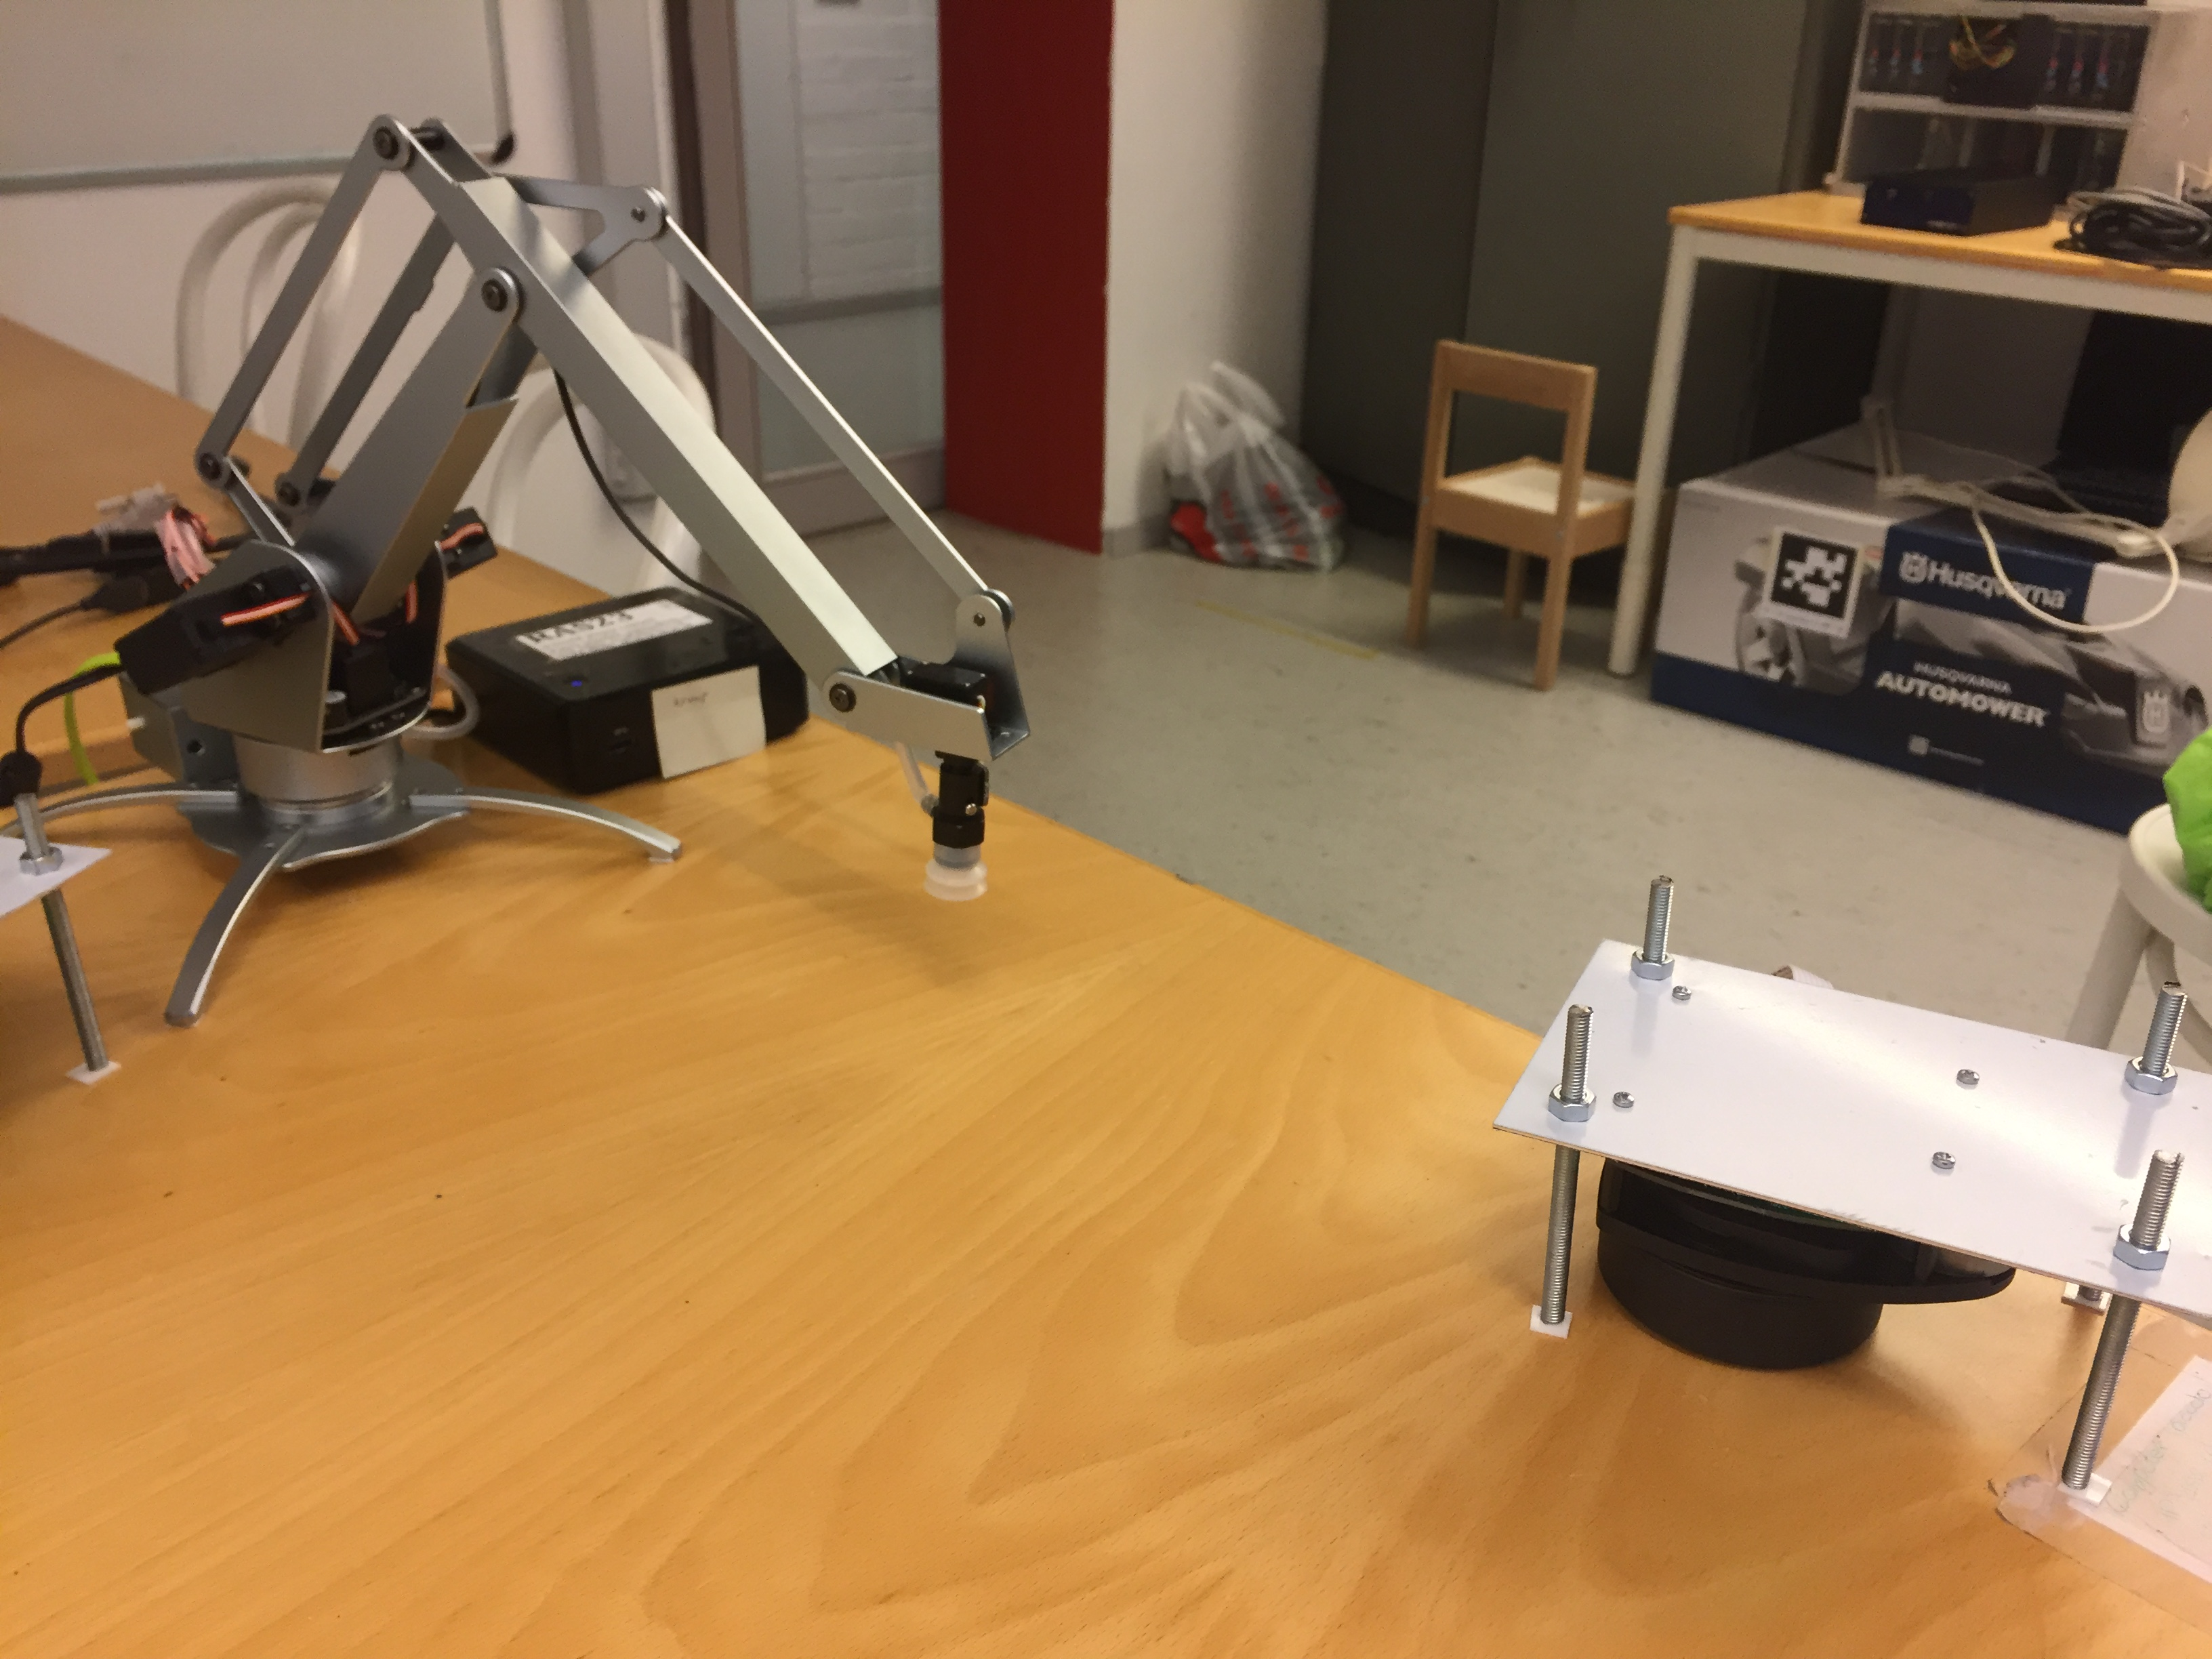
\includegraphics[width=0.48 \textwidth]{res/lidar_placement.JPG}

    \caption{TODO}
    \label{fig:eef-frame}
    
\end{figure}
